\textbf{Входные параметры:}
 
 a --- бинарная строка;
 
 Begin --- номер элемента массива a как начало двоичного числа (начиная с нуля);
 
 n --- длина двоичного числа (это не длина вектора a).
 
\textbf{Возвращаемое значение:}

 Число в десятичной системе исчисления. Если не удается вычислить, то возвращается -1.
 
\textbf{О функции:}

 Для декодирования из бинарной строки берется только часть:
 
 \begin{figure} [h]
  \center
  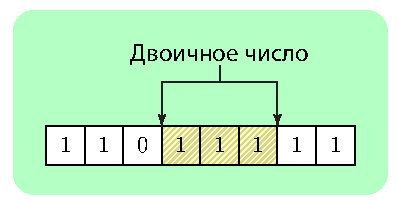
\includegraphics [scale=1] {HML_BinaryToDecimalFromPart_Sheme}
  \caption{Часть бинарной строки} 
  \label{img:HML_BinaryToDecimalFromPart_Sheme}  
\end{figure}
 
 \textbf{Примечание:}
 
 Для перевода всей бинарной строки в число лучше воспользоваться функцией HML\_BinaryToDecimal.

\textbf{Примечание:}

 Данная функция используется, например, если в бинарной строке закодировано несколько десятичных чисел, каждое из которых закодировано своей подстрокой, а общая строка получена склейкой этих бинарных строк.